\section{Bildkompression} \label{sec:compression}
\begin{tcolorbox}
	\centerline{\textbf{Lernziele Kapitel~\ref{sec:compression}}}
	\begin{enumerate}[leftmargin=*,label=\thesection.\arabic*]
		\item \textit{Verstehen}, was die Eigengesichter im Vergleich zu anderen Basen des Gesichtsraumes auszeichnet.
		\item \textit{Erklären} können, wie man die Eigengesichter zur Bildkompression verwenden kann.
		\item Mit gegebenen Eigengesichtern eine Bildkompression in Python implementieren können, falls alle Bilder als Vektoren gegeben sind.
	\end{enumerate}
\end{tcolorbox}
Wenn wir ein schwarz-weiss Bild mit der Auflösung $M=144$ mal $N=180$ Pixel für Pixel abspeichern, so müssen wir $M\cdot N=25920$ Zahlen abspeichern.
Unter Bildkompression versteht man Verfahren, die Bilder mit weniger Zahlen darstellen können.
Das ist zum Beispiel nützlich wenn man Bilder über das Internet verschicken möchte (oder gleich ganze Filme).
Die Datenmenge kann durch Kompression stark verringert werden, was zu viel kürzeren Download-Zeiten führt.
Mit den Eigengesichtern lassen sich Bilder von Gesichtern komprimieren.
Grund dafür ist eine spezielle Eigenschaft, welche die Eigengesichter auszeichnet, und dir wir nun untersuchen werden.

Im letzten Kapitel haben wir das Gemälde der Mona Lisa durch eine Projektion als Linearkombination der Eigengesichter und es Durchschnittsgesichtes angenähert.
Dazu mussten wir mit geeigneten Skalarprodukten die Koeffizienten $c_1,\ldots,c_K$ dieser Linearkombination berechnen.
Allerdings hätte man anstatt der Eigengesichter auch direkt die Differenzgesichter $\vec a_1,\ldots,\vec a_K$ der Bilder aus der Datenbank nehmen können.
In diesem Fall würde man einfach andere Koeffizienten erhalten.
Allerdings lassen sich diese nicht so einfach berechnen, da diese Differenzgesichter nicht orthonormal sind.
Man betrachte Abbildung~\ref{fig:mona_lisa_reconstruction} für einen Vergleich der beiden Varianten.
\begin{figure}[ht]
	\centering
	\begin{tabular}{lcr}
		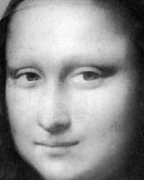
\includegraphics[width=0.2\textwidth]{images/eigenfaces/mona_lisa_naive_approx} &
		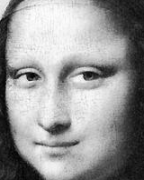
\includegraphics[width=0.2\textwidth]{images/eigenfaces/mona_lisa_original} & 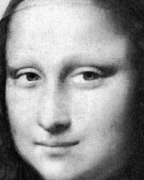
\includegraphics[width=0.2\textwidth]{images/eigenfaces/mona_lisa_eigen_approx}
	\end{tabular}
	\caption{Rekonstruktion der Mona Lisa. Links wurden die Differenzbilder der Testgesichter $\vec a_1,\ldots,\vec a_K$ verwendet. Rechts wurden die Eigengesichter $\vec u_1,\ldots,\vec u_K$ verwendet. In der Mitte ist das Original.}
	\label{fig:mona_lisa_reconstruction}
\end{figure}
Ein weiterer Unterschied zwischen diesen beiden Ansätzen ist die Verteilung der Beträge der Koeffizienten, also $\lvert c_1\rvert,\ldots,\lvert c_K\rvert$.
Diese sind in Abbildung~\ref{fig:coef} gezeigt.
\begin{figure}[ht]
	\centering
	\begin{tabular}{lr}
		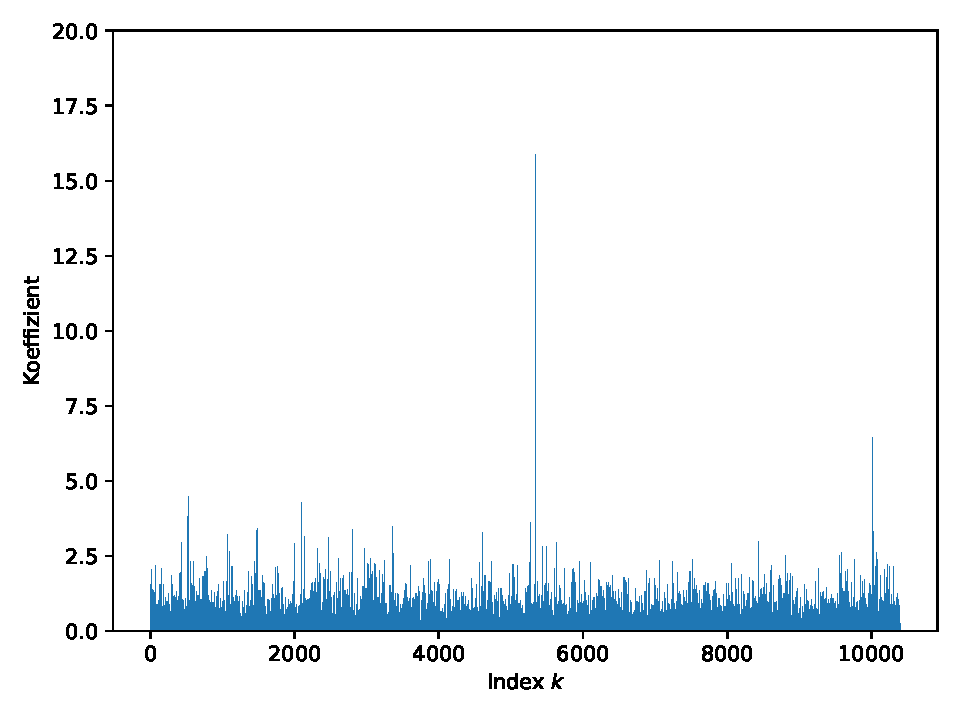
\includegraphics[width=0.45\textwidth]{images/eigenfaces/naive_coef} & 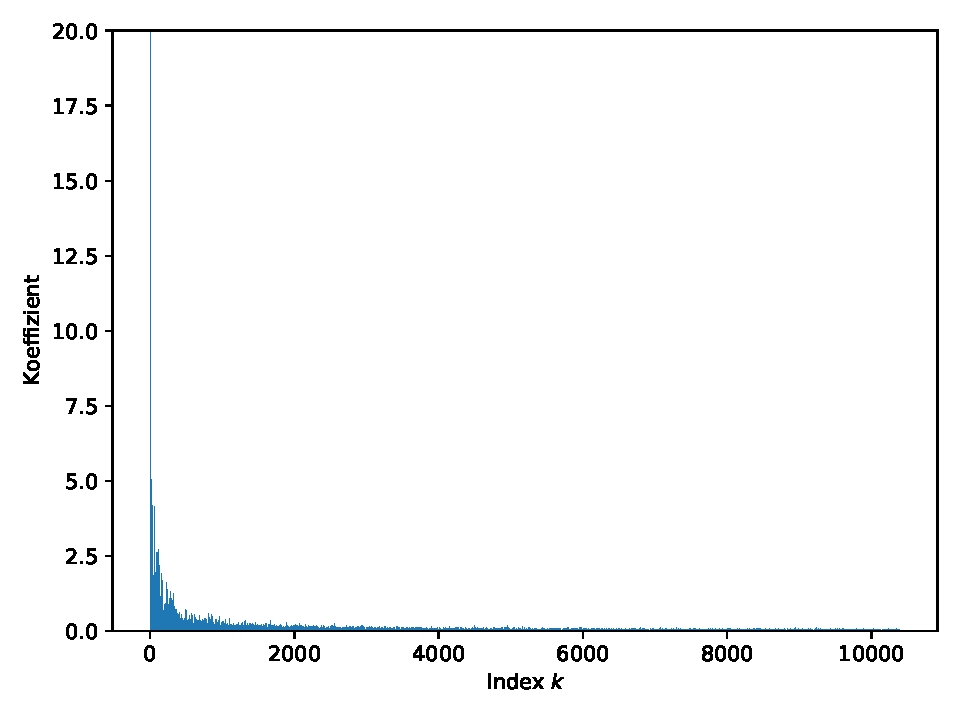
\includegraphics[width=0.45\textwidth]{images/eigenfaces/eigen_coef} \\
	\end{tabular}
	\caption{Der Absolutbetrag der Koeffizienten der Linearkombination des Differenzgesichtes der Mona Lisa, die in Abbildung~\ref{fig:mona_lisa_reconstruction} verwendet wurden. Links die Differenzgesichter der Datenbank und rechts die Eigengesichter verwendet.}
	\label{fig:coef}
\end{figure}
\begin{aufgabe} \label{aufg:coef}
	Betrachten Sie die Abbildung~\ref{fig:coef}, welche die Koeffizienten der Linearkombinationen zeigt, die für die Bilder links bzw. rechts in Abbildung~\ref{fig:mona_lisa_reconstruction} verwendet wurden.
	Beschreiben Sie die Unterschiede in der Verteilung der Koeffizienten.
	Welche Rückschlüsse kann man dadurch ziehen?
\end{aufgabe}
\begin{losung*}
	Die Koeffizienten der Eigengesichter fallen schnell ab.
	Dem rechten Bild kann man entnehmen, dass ungefähr die ersten 2000 Eigengesichter fast den ganzen Beitrag zur Linearkombination leisten.
	Bei der Basis der Differenzgesichter ist keine solche Struktur zu erkennen.
	In diesem Sinn sind alle diese Differenzgesichter etwa gleich wichtig um das Bild der Mona Lisa darstellen zu können.
\end{losung*}
Was wir hier in Abbildung~\ref{fig:coef} beobachtet haben ist kein Einzelfall.
Obwohl wir nur das Beispiel der Mona Lisa betrachtet haben, würden andere Gesichter ähnlich verteilte Koeffizienten liefern.
Die Lösung der vorherigen Aufgabe ist zugleich die Grundidee der Bildkompression mittels Eigengesichter.
Anstatt alle der $K$ Eigengesichter, verwendet man nur die ersten $\tilde K$ Eigengesichter um ein Bild darzustellen.
Die Abbildung~\ref{fig:coef} lässt vermuten, dass wenn $\tilde K$ gross genug gewählt ist, aber immer noch viel kleiner als $K$, sich die Bildqualität nicht wesentlich verschlechtert.
Genauer gesagt, können wir ablesen, dass wohl die ersten $\tilde K=2000$ Eigengesichter ausreichend sein sollten.
Nun wollen ein Bild $\vec p$ rekonstruieren, indem wir nur die ersten $\tilde K$ Eigengesichter verwenden.
Das rekonstruierte Gesicht bezeichnen wir mit $\vec a$, also
\begin{equation*}
	\vec a=\vec m+c_1\vec u_1+c_2\vec u_2+\ldots+c_{\tilde K}\vec u_{\tilde K},
\end{equation*}
wobei $\tilde K\leq K$ und $\vec u_1,\ldots,\vec u_{\tilde K}$ sind die ersten $\tilde K$ Eigengesichter.
Wie man die Koeffizienten $c_1,\ldots,c_{\tilde K}$ berechnet, haben wir im letzten Kapitel gesehen.
\begin{aufgabe}
	Ergänzen Sie die Funktion \texttt{compress(p, m, u\_list, K\_tilde)}, welche einen Vektor der Länge $M\cdot N$ zurück gibt, der dem Bild $\vec a$ entspricht.
	Hier bezeichnen \texttt{p} das ursprüngliche Bild $\vec p$ und \texttt{m} das Durchschnittsgesicht $\vec m$.
	Die Liste \texttt{u\_list} enthält die Eigengesichter und \texttt{K\_tilde} entspricht der Anzahl $\tilde K$ der Eigengesichter, die verwendet werden sollen.
	Testen Sie ihre Lösung indem Sie das Skript \texttt{compress.py} laufen lassen, welches die rekonstruierten Bilder ausgibt.
	\textit{Hinweis:} Verwenden Sie in ihrem Code die Funktion \texttt{compute\_coefficients(p, m, u\_list)} aus Aufgabe~\ref{aufg:compute_coefficients}.
\end{aufgabe}
\begin{losung*}
	Die Lösung könnte zum Beispiel so aussehen.
\begin{lstlisting}[style=python]
import numpy as np

def compress(p, m, u_list, K_tilde):
	# Reduzierte Liste der ersten K_tilde Eigengesichter
	u_list_reduced = u_list[:K_tilde]
	c_list_reduced = compute_coefficients(p, m, u_list_reduced)
	a = np.dot(u_list_reduced, c_list_reduced)
	return a
\end{lstlisting}
Die durch \texttt{compress.py} generierten Bilder sind in Abbildung~\ref{fig:compression} gezeigt.
\end{losung*}
\begin{figure}[ht]
	\centering
	\begin{tabular}{cccc}
		$\tilde K=20$ & $\tilde K=200$ & $\tilde K=2000$ & Original \\
		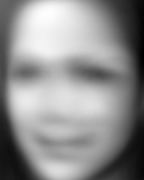
\includegraphics[width=0.1\textwidth]{images/compression/mona_lisa_20} &
		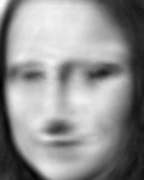
\includegraphics[width=0.1\textwidth]{images/compression/mona_lisa_200} &
		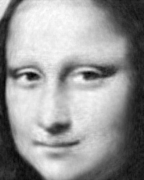
\includegraphics[width=0.1\textwidth]{images/compression/mona_lisa_2000} & 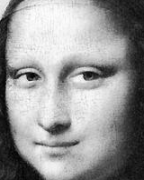
\includegraphics[width=0.1\textwidth]{images/compression/mona_lisa} \\
		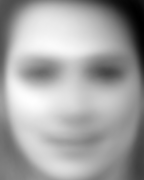
\includegraphics[width=0.1\textwidth]{images/compression/queen_elizabeth_20} &
		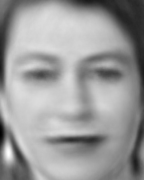
\includegraphics[width=0.1\textwidth]{images/compression/queen_elizabeth_200} &
		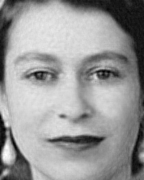
\includegraphics[width=0.1\textwidth]{images/compression/queen_elizabeth_2000} & 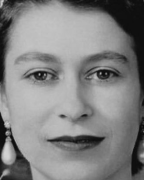
\includegraphics[width=0.1\textwidth]{images/compression/queen_elizabeth} \\
		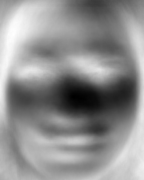
\includegraphics[width=0.1\textwidth]{images/compression/chair_20} &
		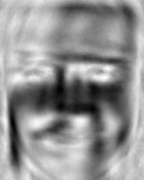
\includegraphics[width=0.1\textwidth]{images/compression/chair_200} &
		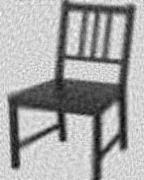
\includegraphics[width=0.1\textwidth]{images/compression/chair_2000} & 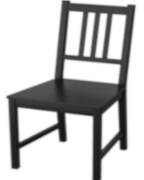
\includegraphics[width=0.1\textwidth]{images/compression/chair} \\
		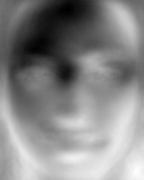
\includegraphics[width=0.1\textwidth]{images/compression/columbia_20} &
		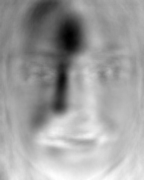
\includegraphics[width=0.1\textwidth]{images/compression/columbia_200} &
		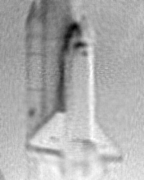
\includegraphics[width=0.1\textwidth]{images/compression/columbia_2000} & 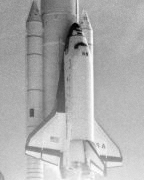
\includegraphics[width=0.1\textwidth]{images/compression/columbia}
	\end{tabular}
	\caption{Rekonstruktion mit verschiedenen $\tilde K$. Gezeigt sind die Mona Lisa, Queen Elizabeth, ein Stuhl und das erste Space Shuttle \glqq{}Columbia\grqq{}. Gesichter werden generell besser rekonstruiert als andere Bilder.}
	\label{fig:compression}
\end{figure}
Was wir in Abbildung~\ref{fig:compression} beobachten ist eine Bildkompression.
Sind die Eigengesichter bekannt, so lässt sich ein Bild rekonstruieren aus den Koeffizienten $c_1,\ldots,c_{\tilde K}$ der ersten $\tilde K$ Eigengesichter.
Um ein Bild eines Gesichtes in leicht verminderter Qualität über das Internet zu versenden, wäre es ausreichend, nur $\tilde K=2000$ Zahlen zu versenden, sofern der Empfänger über die Eigengesichter verfügt.
Wir erinnern uns, dass ein Bild welches Pixelweise versendet wird, $M\cdot N=25920$ Zahlen benötigt.
Das ist etwa ein Faktor 13 mehr als die komprimierte Variante.
Trotzdem sieht man für $\tilde K=2000$ kaum einen Unterschied zum Original in Abbildung~\ref{fig:compression}.
Gleichzeitig sehen wir, dass die aggressivere Komprimierung mit $\tilde K=200$ die Bildqualität doch sehr vermindert.
Aber das konnte man aufgrund des rechten Verteilung in Abbildung~\ref{fig:coef} schon vermuten.
Die linke Verteilung zeigt zugleich, dass dies mit der Basis der Differenzgesichter nicht möglich gewesen wäre.
Weiter beobachten wir, dass die Komprimierung für Bilder, welche kein Gesicht zeigen, weniger gut funktioniert.
Der Grund dafür ist, das andere Differenzbilder nicht notwendigerweise nahe am Raum der Differenzgesichter liegen.
Doch die Eigengesichter sind eine Basis eben dieses Unterraumes.